\section{Introduction}
\label{sec:intro}
Vision-Language Models (VLMs) \cite{clip, align, flamingo, filip, kosmos1, kosmos2, vila}, such as CLIP \cite{clip}, have gained significant attention for their ability to leverage the rich, complementary information inherent in both textual and visual modalities. By constructing distinct encoders for images and text, and employing contrastive learning \cite{contrastive_learning} on over 400 million image-text pairs, CLIP effectively captures complex visual-text relationships, demonstrating strong performance across various downstream tasks, such as medical image analysis \cite{clip_medical1, clip_medical2, clip_medical3}, image and video captioning \cite{clip_captioning1, clip_captioning2, clip_captioning3}, and visual question answering \cite{clip_answering1, clip_answering2, clip_answering3}. Despite their versatility, VLMs encounter limitations in adapting to new tasks, as fine-tuning their large-scale architectures demands considerable computational resources.

%-------------------------------------------------------------------------


\begin{figure}[tb]
\centering
\setlength{\abovecaptionskip}{0.2cm}   %调整图片标题与图距离
  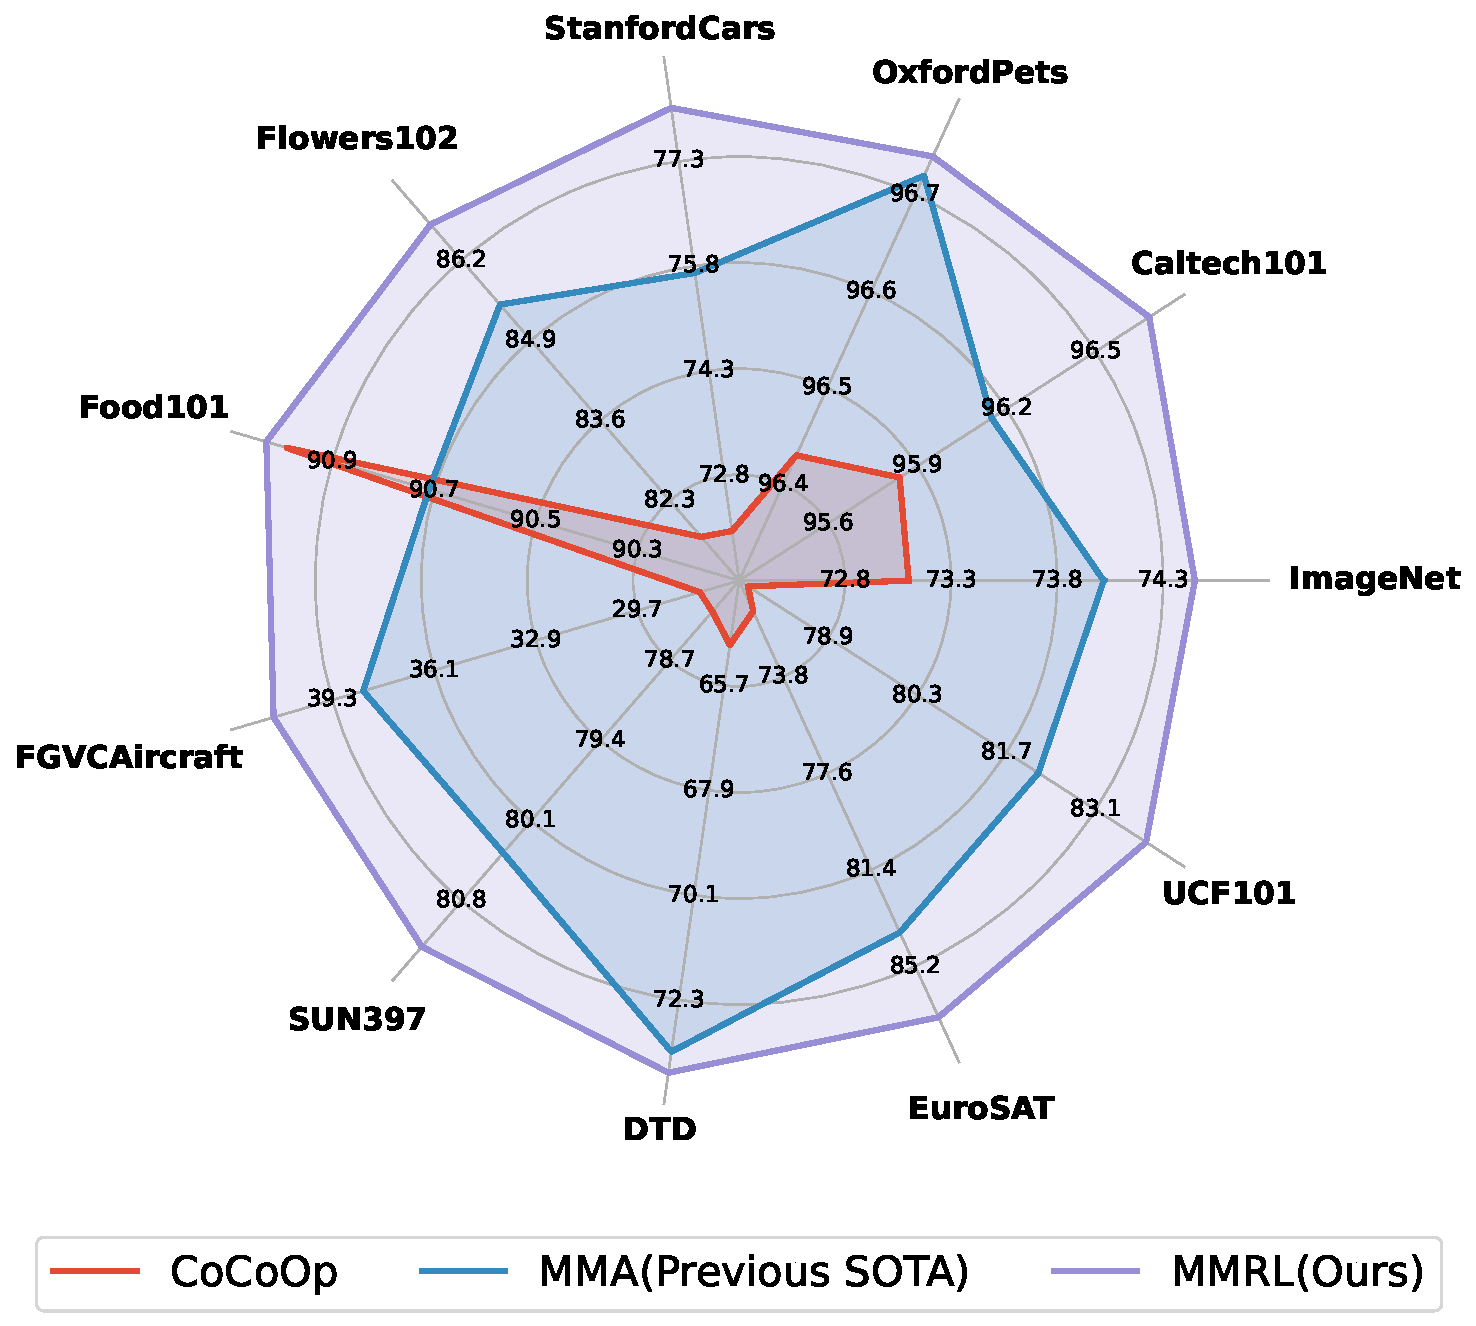
\includegraphics[width=0.9\linewidth]{fig/radar.pdf}
  \caption{Comprehensive comparison of the harmonic mean performance between the previous sota method MMA and our proposed MMRL across 11 diverse datasets for base-to-novel generalization. Our method achieves the best on all datasets.}
  \label{radar}
\vspace{-0.5cm}
\end{figure}
%-------------------------------------------------------------------------

To facilitate efficient adaptation of VLMs, strategies such as prompt engineering and ensembling \cite{clip} have shown potential. Specifically, prompt engineering involves crafting dataset-specific prompts, such as ``A photo of a [CLASS], a type of pet.'' for the OxfordPets \cite{oxford_pets} dataset. Alternatively, ensembling can integrate multiple zero-shot classifiers by varying context prompts, \eg, ``A photo of a big [CLASS].'' and ``A photo of a small [CLASS].''. Nonetheless, manual prompt design is time-consuming and requires substantial expertise, yet it does not guarantee the discovery of optimal prompts. To address this limitation, CoOp \cite{coop} introduces prompt learning\cite{prompt_tuning} where prompts are modeled as continuous learnable vectors, optimized during training while keeping VLM parameters fixed, thereby enabling efficient dataset adaptation. Recently MaPLe \cite{maple} has identified that prompt learning solely within the text modality may be sub-optimal. In response, it proposes a multi-modal prompt learning approach, embedding deep prompts into the lower layers of both VLM encoders via a coupling function to enhance alignment between visual and textual representations.

In addition to prompt learning, adapter-style learning methods offer a different adaptation pathway: rather than modifying input prompts, lightweight modules (\eg, multi-layer perceptrons, MLPs) are integrated within VLMs to adjust extracted features for downstream datasets. CLIP-Adapter \cite{clip-adapter} exemplifies this approach by maintaining the frozen VLM while fine-tuning features via an MLP adapter added to the image encoder, which incorporates residual connections for feature fusion. Similar to MaPLe, MMA \cite{mma} proposes a multimodal adapter that refines the alignment between text and vision representations by aggregating features from diverse branches into a unified feature space, allowing gradient flow across branches. Notably, MMA reveals that different layers within VLM encoders capture varying characteristics: higher layers encode discriminative, dataset-specific information, while lower layers retain more generalizable features.

However, the current multimodal deep prompt learning method \cite{maple}, which applies prompt concatenation at shallow layers, may compromise generalizable knowledge. This approach map visual prompts from text prompts, incorporating visual information via gradient propagation but ultimately remaining text-centric, with updates focused mainly on text prompts. Moreover, both prompt learning and adapter-style methods solely optimize class token features using task-specific objectives, such as cross-entropy loss. As a result, these methods are vulnerable to overfitting to specific data distributions or task categories when training data is scarce (\eg, few-shot setting), leading to a decline in the inherent generalization and zero-shot learning capabilities of VLMs.


To address these challenges, we propose a novel multi-modal representation learning framework that distinguishes itself from conventional prompt learning and adapter-style methods. Specifically, we introduce a shared, learnable representation space that is independent of any modality within the higher layers of the encoder. This space serves as a bridge for multimodal interaction, mapping tokens from this space to both image and text representation tokens, which are then concatenated with the original encoder tokens to enable effective multimodal interaction. Our representation tokens are designed to learn dataset-specific knowledge from downstream tasks while the original classification token is regularized to retain a significant amount of generalizable knowledge. MMRL offers three key advantages: (1) an unbiased shared representation space that promotes balanced multimodal learning; (2) preservation of original VLM generalization by avoiding prompt integration at shallow encoder layers; and (3) Unlike prompt learning or adapter-style methods that refine only the class token features through learnable prompts or adapters, our approach supports decoupled inference across classes. During training, we prioritize optimizing representation token features, with their projection layer trainable, while that of the original class token remain fixed. To further preserve the generalizability of the class token, a regularization term aligns its features with the zero-shot features from the frozen VLM. For inference, we utilize both representation and class token features for base classes, while for unseen classes or new datasets, only the class token features are employed.


Our main contributions are summarized as follows:
\begin{itemize}
    \item We introduce the \textbf{M}ulti-\textbf{M}odal \textbf{R}epresentation \textbf{L}earning (MMRL) framework, which incorporates a shared, unbiased, learnable space that bridges image and text modalities, facilitating multimodal interaction at the high layers of the original encoder.
    \item A decoupling strategy preserves VLM generalization by adapting representation tokens for downstream tasks while regularizing the original class token for new tasks.
    \item Extensive experiments demonstrate that MMRL substantially improves downstream adaptation and generalization, achieving superior performance over baselines.
\end{itemize}



%-------------------------------------------------------------------------


\begin{figure*}
\centering
\setlength{\abovecaptionskip}{0.2cm}   %调整图片标题与图距离
  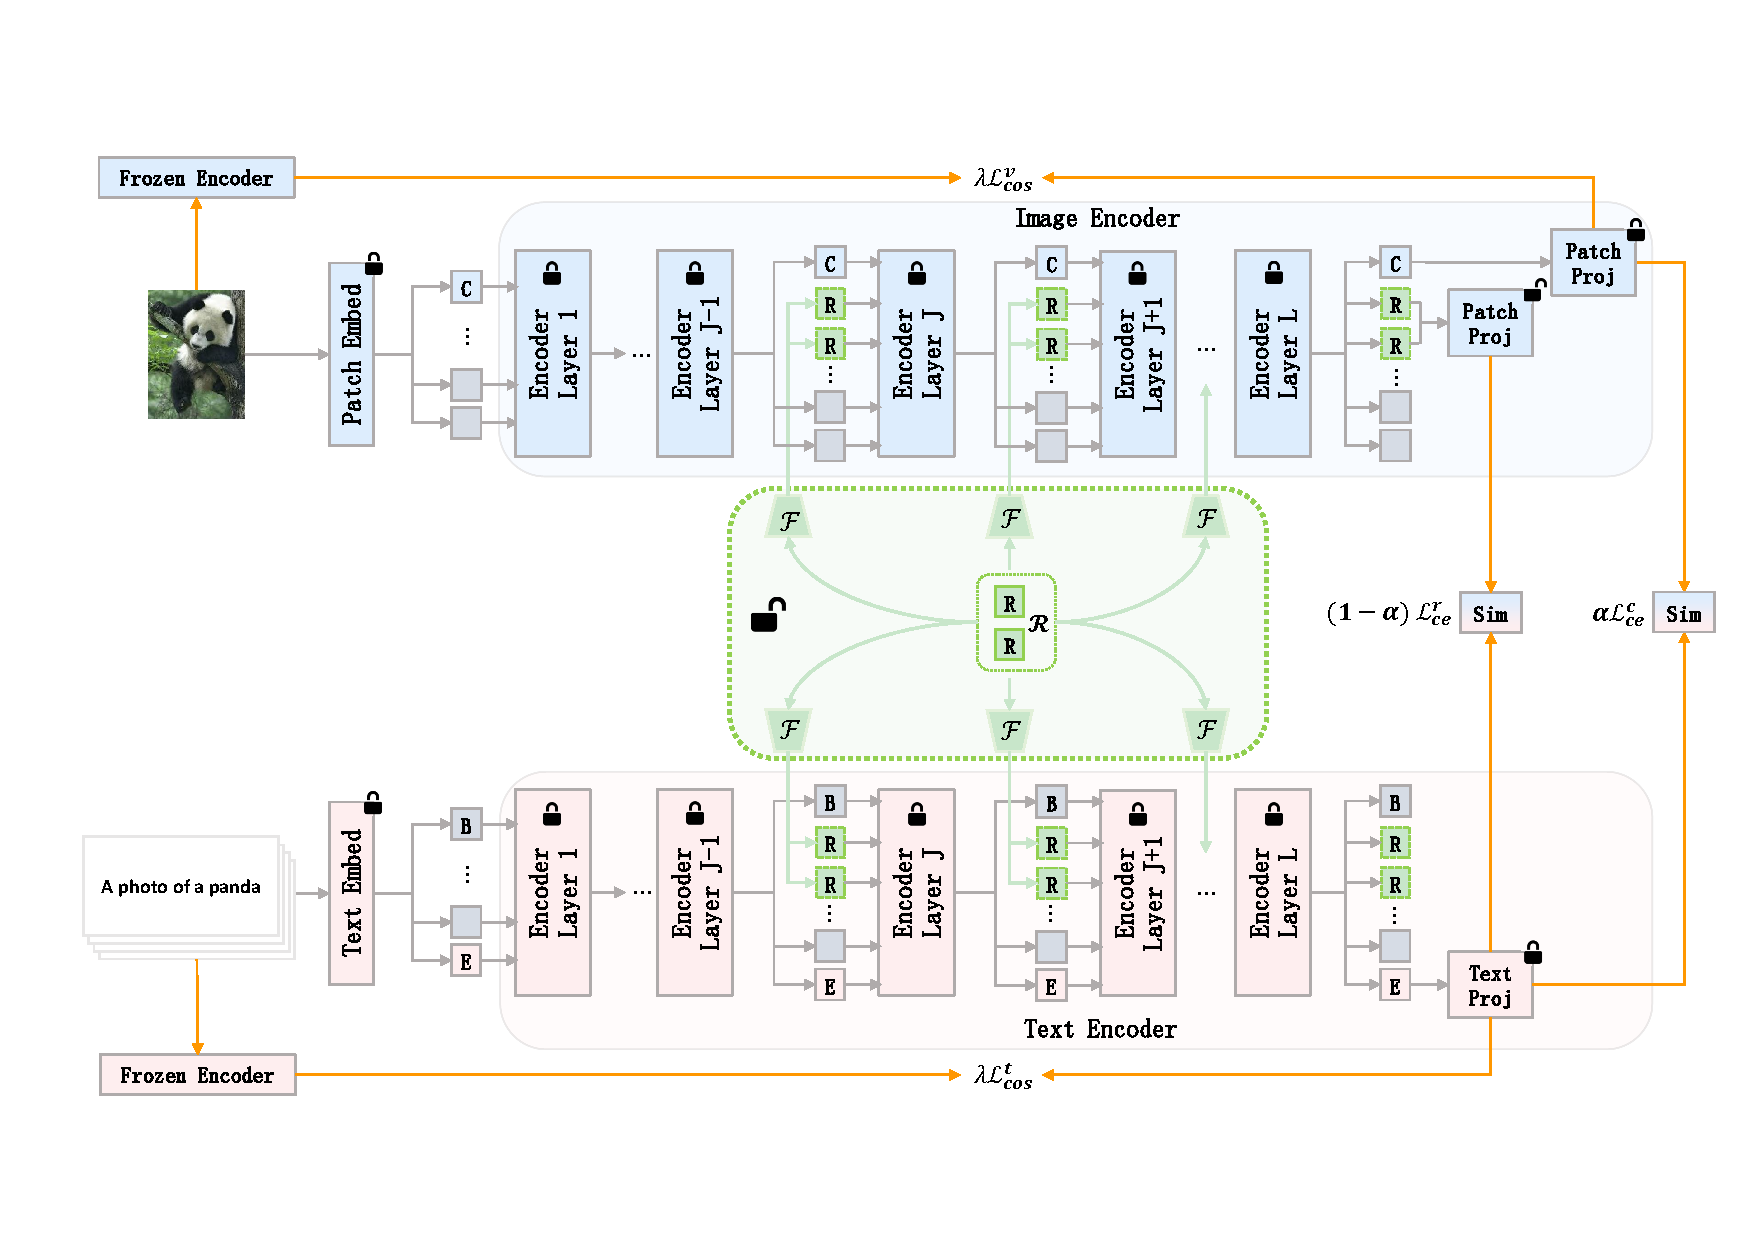
\includegraphics[width=0.9\linewidth]{fig/frame1.pdf}
  \caption{MMRL training framework. Here, `C' denotes the class token, `B' the BOT token, `E' the EOT token, $\mathcal{R}$ our representation space, and `R' the representation token. Only the representation space $\mathcal{R}$, mapping function $\mathcal{F}$, and the patch projection layer for the representation tokens are optimized, while the entire pre-trained CLIP model remains frozen. To preserve generalization knowledge, we integrate representation tokens in both encoders starting from layer $J$.}
  \label{framework1}
\vspace{-0.5cm}
\end{figure*}

